\section{Points}
\subsection{Comparing floating point values}
Returns true if double values a and b are equal
\cppscript{geometry/src/equals}{equals}


\section{Lines}
\subsection{General equation of a line}
Non-normalized form: ax + by + c = 0
\cppscript{geometry/src/line_general}{General equation of a line}

\subsection{General equation of a line normalized}
\cppscript{geometry/src/line_general_normalized}{General equation of a line}

\subsection{Point on a line}
Is the given point located on the given Line?
\cppscript{geometry/src/line_contains}{Point on line}

\subsection{Equal and parallel lines}
\cppscript{geometry/src/parallel}{}

\subsection{Orthogonal}
\cppscript{geometry/src/orthogonal}{}

\subsection{Intersection}
\cppscript{geometry/src/intersection}{}

\subsection{Angle between lines}
\cppscript{geometry/src/angle_lines}{}

\subsection{Distance to point}
\cppscript{geometry/src/distance_line_point}{}

\subsection{Bissector / Mediatriz}
\cppscript{geometry/src/mediatriz}{}

\subsection{Orientation between point and line}
\cppscript{geometry/src/D}{}

\section{Line segments}

\subsection{Contains point}
\cppscript{geometry/src/segment_contains}{}

\subsection{Closest point}
\cppscript{geometry/src/segment_closest}{}

\subsection{Intersectin with segment}
\cppscript{geometry/src/segment_intersection}{}

\section{Vectors}

\subsection{Angle between vector and X-axis}
Returns an angle in radians in the interval $\interval{-\pi}{+\pi}$. A positive angle means in the COUNTER-clockwise direction. A negative angle is measured in the clockwise direction. Note that the atan2 swaped the parameters.
\cppscript{geometry/src/angle}{angle between X-axis and vector{x, y}}

\subsection{Translation}
\cppscript{geometry/src/translation}{Translate point}

\subsection{Rotation around origin}
\cppscript{geometry/src/rotation}{}

\subsection{Rotation around another point}
\cppscript{geometry/src/rotation_point}{}

\subsection{Rotation around origin 3D}

\begin{center}
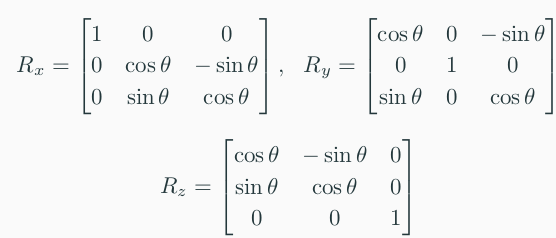
\includegraphics[width = 7in, height = 3.5in]{geometry/images/rotation3d.png}
\end{center}

\subsection{Scale}
\cppscript{geometry/src/scale}{Scale vector by a factor of sx and sy}

\subsection{Normalization}
\cppscript{geometry/src/normalize}{Returns a unit vector with the same direction as the given vector}

\subsection{Dot product}
\[
    <\vec{u}, \vec{v}> = \vec{u} \cdot \vec{v} = u_xv_x + u_yv_y = |\vec{u}||\vec{v}|\cos \theta
\]

\cppscript{geometry/src/dot}{}

\subsection{Angle between vectors}
\cppscript{geometry/src/angle_vectors}{}

\subsection{Cross product}

$
            u\times v = \begin{vmatrix}
                \vec{i} & \vec{j} & \vec{k} \\
                u_x & u_y & u_z \\
                v_x & v_y & v_z \\
            \end{vmatrix}
$
\begin{itemize}
\item $|\vec{u}\times \vec{v}| = |\vec{u}||\vec{v}|\sin \theta$
\item where $\vec{i}, \vec{j}, \vec{k}$ are unity vectors on the same direction and orientation as $x, y, z$, respectively
\item the result vector $\vec{w}$ is orthogonal to both $\vec{u}$ and $\vec{v}$
\item it is the area of the parallelogram formed by $\vec{u}$ and $\vec{v}$
\end{itemize}

\cppscript{geometry/src/cross}{}

\section{Circles}

\subsection{Definition}
\cppscript{geometry/src/circle_definition}{}

\subsection{Perimeter, Area}
\cppscript{geometry/src/circle_perimeter}{}

\subsection{From 2 points}
\cppscript{geometry/src/circle_from_2_points}{}

\subsection{From 3 points}
\cppscript{geometry/src/circle_from_3_points}{}

\clearpage
